\documentclass[]{article}
\usepackage{lmodern}
\usepackage{amssymb,amsmath}
\usepackage{ifxetex,ifluatex}
\usepackage{fixltx2e} % provides \textsubscript
\ifnum 0\ifxetex 1\fi\ifluatex 1\fi=0 % if pdftex
  \usepackage[T1]{fontenc}
  \usepackage[utf8]{inputenc}
\else % if luatex or xelatex
  \ifxetex
    \usepackage{mathspec}
  \else
    \usepackage{fontspec}
  \fi
  \defaultfontfeatures{Ligatures=TeX,Scale=MatchLowercase}
\fi
% use upquote if available, for straight quotes in verbatim environments
\IfFileExists{upquote.sty}{\usepackage{upquote}}{}
% use microtype if available
\IfFileExists{microtype.sty}{%
\usepackage{microtype}
\UseMicrotypeSet[protrusion]{basicmath} % disable protrusion for tt fonts
}{}
\usepackage[margin=1in]{geometry}
\usepackage{hyperref}
\hypersetup{unicode=true,
            pdftitle={Igor Portnoy's CV},
            pdfauthor={Igor Portnoy},
            pdfborder={0 0 0},
            breaklinks=true}
\urlstyle{same}  % don't use monospace font for urls
\usepackage{graphicx,grffile}
\makeatletter
\def\maxwidth{\ifdim\Gin@nat@width>\linewidth\linewidth\else\Gin@nat@width\fi}
\def\maxheight{\ifdim\Gin@nat@height>\textheight\textheight\else\Gin@nat@height\fi}
\makeatother
% Scale images if necessary, so that they will not overflow the page
% margins by default, and it is still possible to overwrite the defaults
% using explicit options in \includegraphics[width, height, ...]{}
\setkeys{Gin}{width=\maxwidth,height=\maxheight,keepaspectratio}
\IfFileExists{parskip.sty}{%
\usepackage{parskip}
}{% else
\setlength{\parindent}{0pt}
\setlength{\parskip}{6pt plus 2pt minus 1pt}
}
\setlength{\emergencystretch}{3em}  % prevent overfull lines
\providecommand{\tightlist}{%
  \setlength{\itemsep}{0pt}\setlength{\parskip}{0pt}}
\setcounter{secnumdepth}{0}
% Redefines (sub)paragraphs to behave more like sections
\ifx\paragraph\undefined\else
\let\oldparagraph\paragraph
\renewcommand{\paragraph}[1]{\oldparagraph{#1}\mbox{}}
\fi
\ifx\subparagraph\undefined\else
\let\oldsubparagraph\subparagraph
\renewcommand{\subparagraph}[1]{\oldsubparagraph{#1}\mbox{}}
\fi

%%% Use protect on footnotes to avoid problems with footnotes in titles
\let\rmarkdownfootnote\footnote%
\def\footnote{\protect\rmarkdownfootnote}

%%% Change title format to be more compact
\usepackage{titling}

% Create subtitle command for use in maketitle
\providecommand{\subtitle}[1]{
  \posttitle{
    \begin{center}\large#1\end{center}
    }
}

\setlength{\droptitle}{-2em}

  \title{Igor Portnoy's CV}
    \pretitle{\vspace{\droptitle}\centering\huge}
  \posttitle{\par}
    \author{Igor Portnoy}
    \preauthor{\centering\large\emph}
  \postauthor{\par}
      \predate{\centering\large\emph}
  \postdate{\par}
    \date{2019-10-10}


\begin{document}
\maketitle

\hypertarget{aside}{%
\section{Aside}\label{aside}}

\begin{figure}
\centering
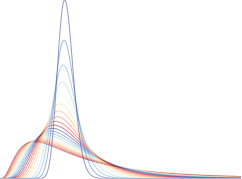
\includegraphics[width=1\textwidth,height=\textheight]{beta_dist.png}
\caption{logo}
\end{figure}

\hypertarget{contact}{%
\subsection{Contact}\label{contact}}

\begin{itemize}
\tightlist
\item
  \href{mailto:Igoryan10@gmail.com}{\nolinkurl{Igoryan10@gmail.com}}
\item
  IgorPortnoy
\item
  github.com/IgorPortnoy
\item
  (+972)54-819-5657
\end{itemize}

\hypertarget{skills}{%
\subsection{Skills}\label{skills}}

Highly experienced in

\begin{itemize}
\tightlist
\item
  R
\item
  SQL
\end{itemize}

Experience with

\begin{itemize}
\tightlist
\item
  git
\item
  python
\item
  C++
\item
  docker
\end{itemize}

\hypertarget{disclaimer}{%
\subsection{Disclaimer}\label{disclaimer}}

Made with the R package
\href{https://github.com/rstudio/pagedown}{\textbf{pagedown}}.

The source code is available at
\href{https://github.com/IgorPortnoy/my-r-cv}{github.com/IgorPortnoyr/my-r-cv}.

Last updated on 2019-10-10.

\hypertarget{main}{%
\section{Main}\label{main}}

\hypertarget{title}{%
\subsection{Igor Portoy}\label{title}}

Experienced Data Science Specialist with a demonstrated history of
working in the computer software industry. Skilled in statistics, R,
Pyhton, SQL. Strong engineering thinking and focused on solving business
problems using different machine learning alogrithems, depending on the
problem.

\hypertarget{education}{%
\subsection{Education}\label{education}}

\hypertarget{m.a-economics}{%
\subsubsection{M.A Economics}\label{m.a-economics}}

Bar-Ilan University

Ramat Gan, ISR

2017 - 2015

\begin{itemize}
\tightlist
\item
  Thesis: Does Financial Development and Reform Spur Economic Growth? A
  Case Study of the Israeli Experience
\end{itemize}

\hypertarget{b.a-economics}{%
\subsubsection{B.A , Economics}\label{b.a-economics}}

Academic college - Bar ilan University extension

Ashkelon, ISR

2010 - 2008

\begin{itemize}
\tightlist
\item
  Graduated with Cum laude
\end{itemize}

\hypertarget{research-experience}{%
\subsection{Research Experience}\label{research-experience}}

\hypertarget{research-assistant}{%
\subsubsection{Research Assistant}\label{research-assistant}}

Technology Analysis and Forecasting Center

Tel-Aviv University

2013

\begin{itemize}
\tightlist
\item
  Participating at European project, RACE 2050, wrote macro reviews
  about the impacts of European Security \& Energy policies on global
  competitiveness of European transport industry.
\end{itemize}

\hypertarget{industry-experience}{%
\subsection{Industry Experience}\label{industry-experience}}

\hypertarget{data-science-tech-lead}{%
\subsubsection{Data Science Tech Lead}\label{data-science-tech-lead}}

Octopol

kfar Saba, ISR

2019 - 2017

\begin{itemize}
\tightlist
\item
  Leading companies data team
\end{itemize}

\hypertarget{data-science}{%
\subsubsection{Data Science}\label{data-science}}

Octopol

kfar Saba, ISR

2017 - 2015

\begin{itemize}
\tightlist
\item
  Responsible for end-to-end delivery of predictive models (from idea to
  production), using machine learning algorithems.
\end{itemize}

\hypertarget{data-analyst}{%
\subsubsection{Data Analyst}\label{data-analyst}}

Delek

Netanya, ISR

2015 - 2013

\begin{itemize}
\tightlist
\item
  Research different business problems, using companies data.
\item
  Worked on developing forecasting models of firm's time series data.
\item
  Provided statistical data analysis like consumer behavior analysis and
  marketing analysis.
\end{itemize}


\end{document}
